
\begin{figure*}
\centering
\begin{tabular}{cccc}
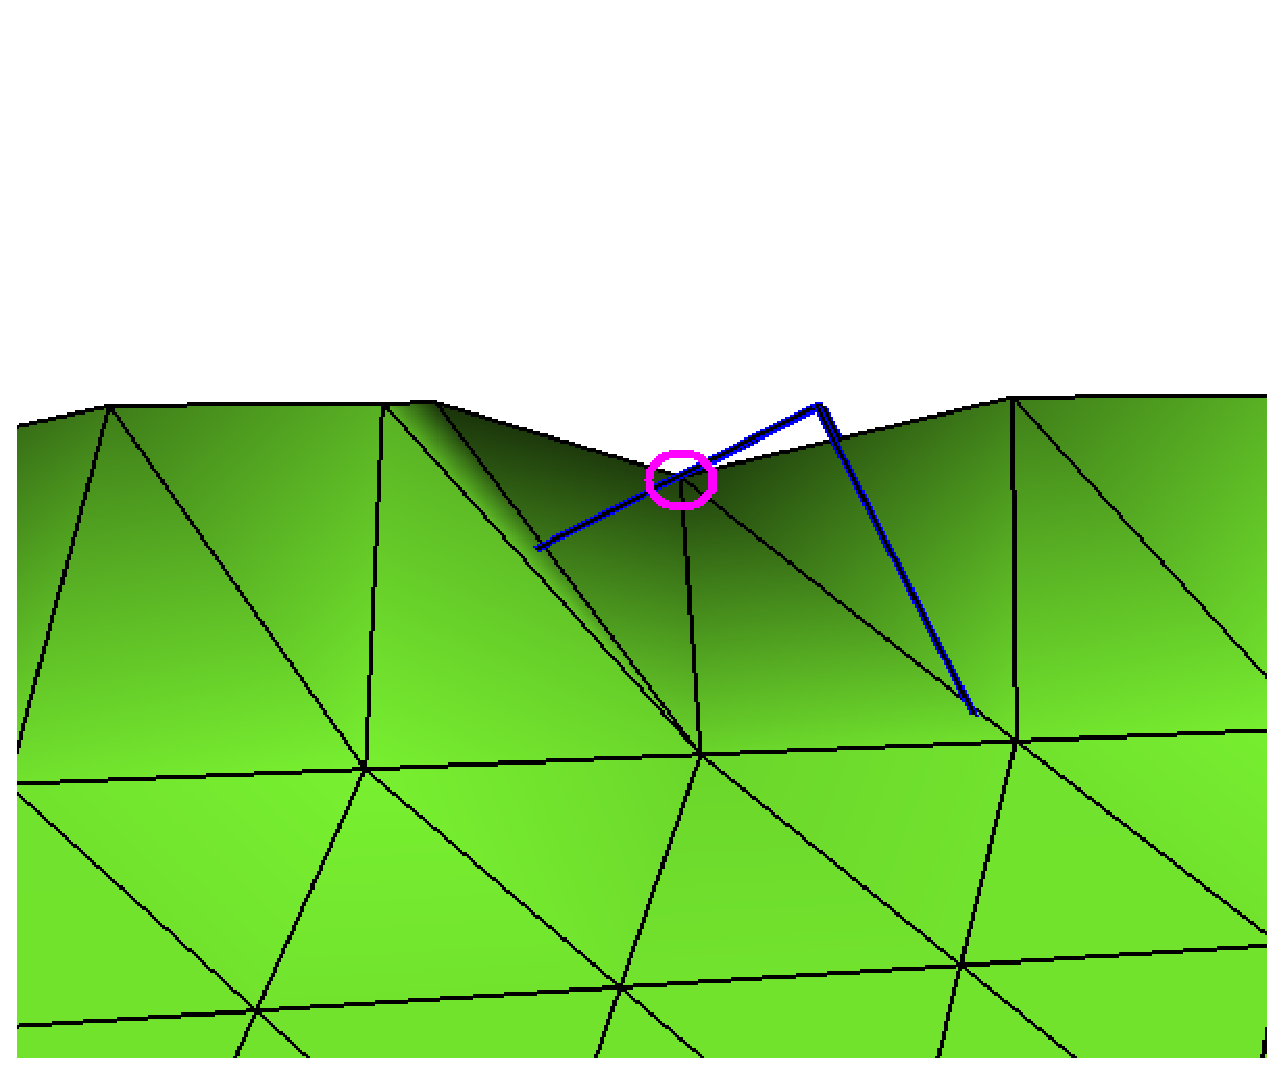
\includegraphics[width=1.2in]{images/cubeA_notch} \qquad &
\qquad
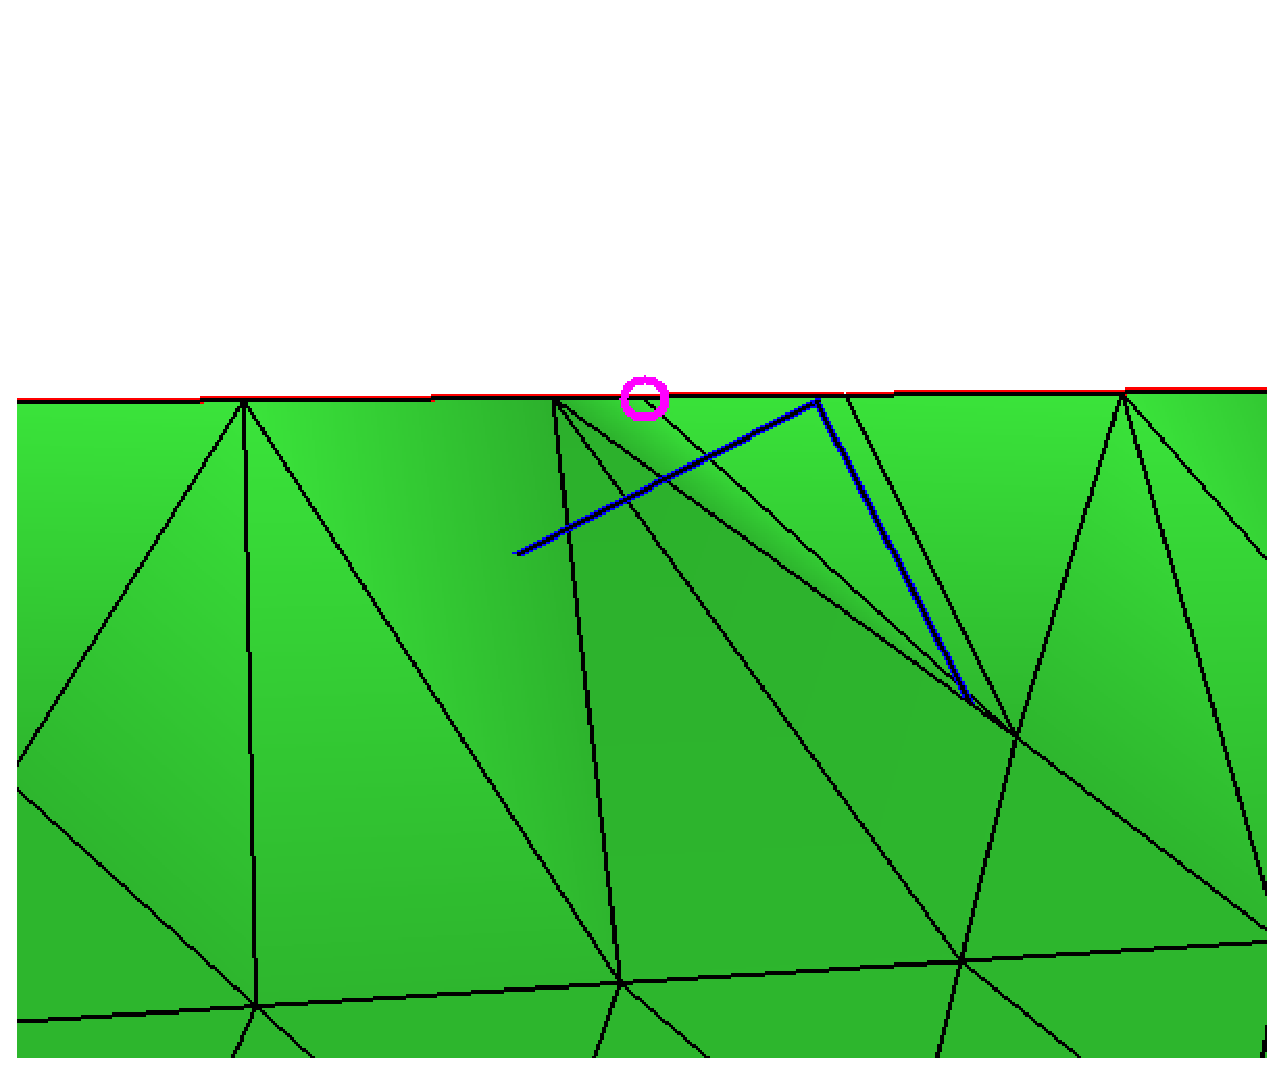
\includegraphics[width=1.2in]{images/cubeA_no_clamp.eps}
\qquad &
\qquad
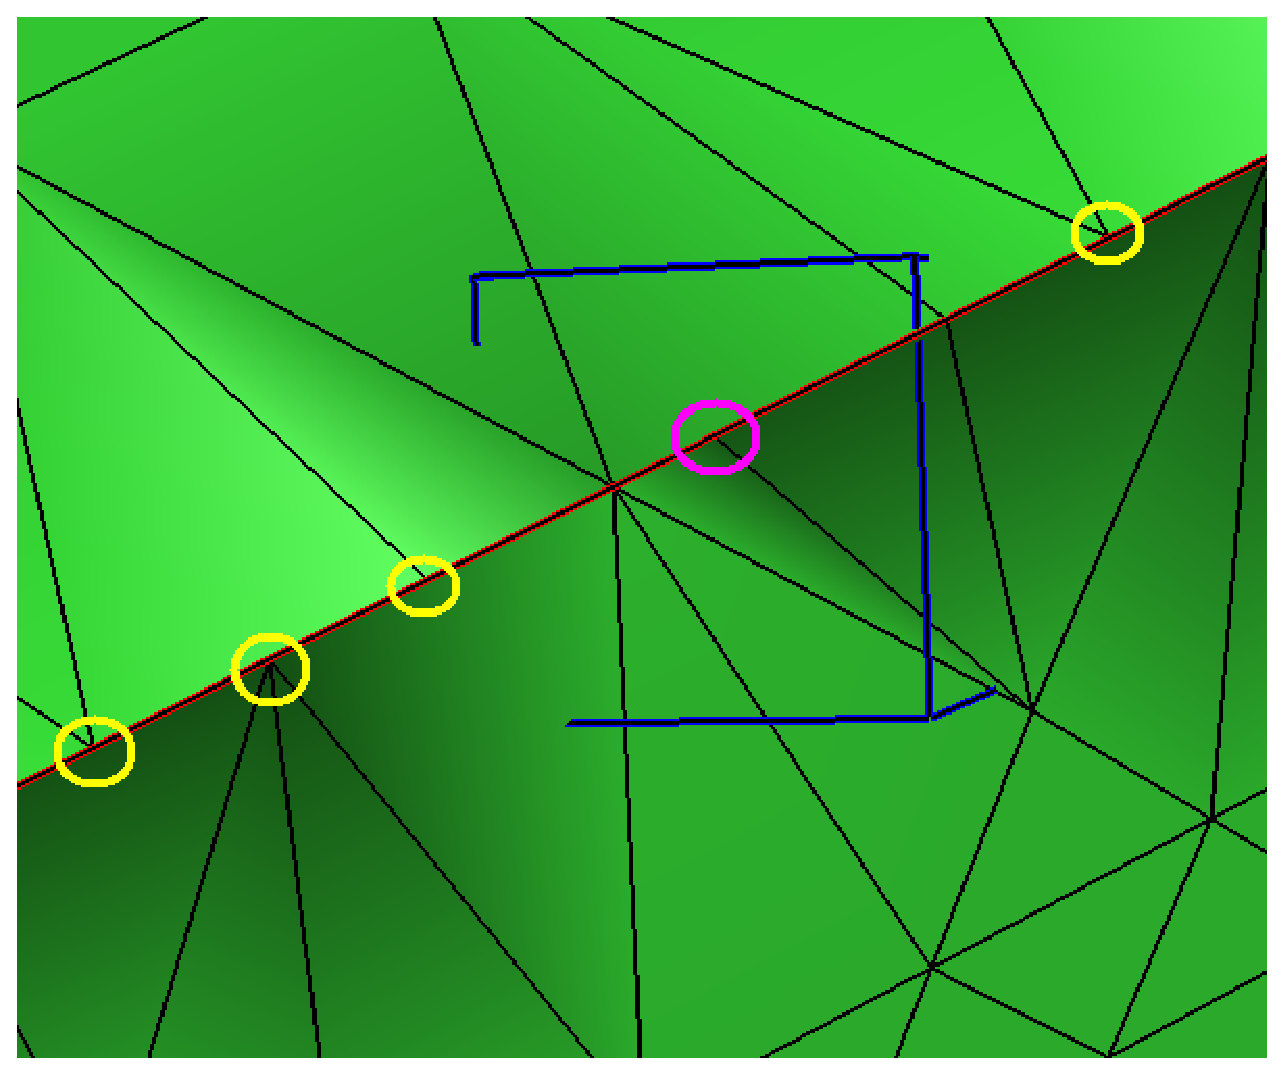
\includegraphics[width=1.2in]{images/cubeA_degen.eps}
\qquad &
\qquad
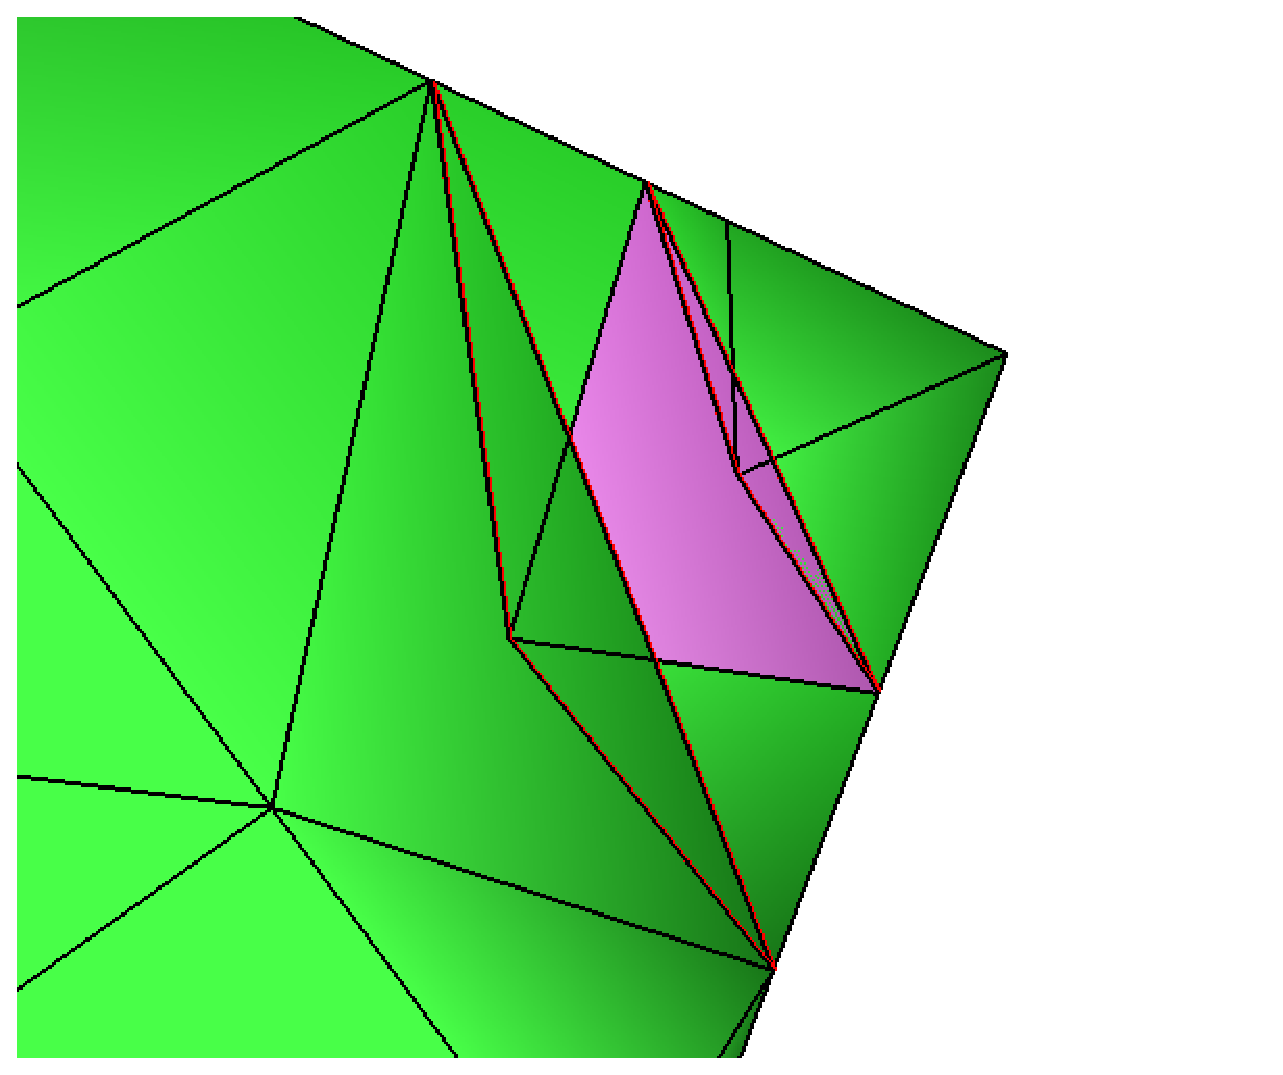
\includegraphics[width=1.2in]{images/mesh_fold_EMC.eps} \\
(a) Notch in 1D feature & (b) Not clamped to cube
  & (c) Degenerate triangles & (d) Folds in mesh \\
\end{tabular}
\caption{Reconstruction problems.
(a)~The orange cube generates the vertex in the magenta circle.
Clamping the vertex to the orange cube creates a notch 
in the 1-dimensional feature.
(b)~Same mesh as (a) but vertex in the magenta circle is not
clamped to the orange cube.
(c)~Different view of mesh, vertex and cube in (b).
The vertex in the magenta circle is part of a degenerate triangles
which lies on the 1D feature.
Vertices in the yellow circles are also part of degenerate triangles
which lie on the 1D feature.
Note that the mesh is fully triangulated so that the apparent
mesh quadrilaterals are actually mesh triangles adjacent 
to degenerate triangles.
(d)~Mesh folds produced by Extended Marching Cubes near a cube corner.
The fold edges are at highlighted in red.
The magenta triangle overlaps six other mesh triangles.}
\label{fig:problems}
\end{figure*}


\section{Related Work}
\label{section:related}

The well-known Marching Cubes algorithm~\cite{lc-mchr3-87}
by Lorensen and Cline
constructs isosurface patches within active grid cubes.
The isosurface patches align along their common boundaries.
Because Marching Cubes positions vertices only on grid edges,
never inside grid cubes,
it does a poor job at representing sharp features on isosurfaces.

Dual contouring algorithms construct an isosurface using quadrilaterals
which are dual to active grid edges.
The isosurface vertices are located within the grid cubes,
not on grid edges.
Gibson~\cite{gh-ssqem-97,g-cesng-98} gave the first dual contouring algorithm
which she called surface nets.
Because Gibson's algorithm placed only one isosurface vertex 
in each active cube,
it produced many isosurface edges contained in four quadrilaterals.
Thus, the resulting isosurface was not a manifold.
Nielson~\cite{n-dmc-04} modified Gibson's algorithm
to allow multiple isosurface vertices in active cubes.
The number of vertices in a grid cube $\cb$
corresponds to the number of isosurface patches in $\cb$
produced by the Marching Cubes algorithm.

Nielson's algorithm eliminates most, but not all, 
of the non-manifold problems in dual contouring.
A dual contouring algorithm
for constructing an isosurface which is a always a manifold
is contained in~\cite{Wenger:2013:Isosurfaces}.
The algorithm is essentially Nielson's algorithm
but the number and connectivity of isosurface vertices in grid cubes
is sometimes modified.

In~\cite{l-oslpm-00}, Lindstrom gave an algorithm for locating a point 
on a surface from a set of $n$ tangent planes.
The $n$ tangent give a set of $n$ equations in three unknowns,
described by $M x = b$ where $M$ is an $n \times 3$ matrix 
and $b$ is a column vector of length $n$.
Lindstrom uses the singular valued decomposition (SVD) of $M$
to determine a point close to all the tangent planes.
The SVD of $M$ also indicates whether the point is
on a 0-dimensional (corner) or 1-dimensional (edge) surface feature
or on a smooth portion of the surface.
Lindstrom's algorithm is described in more detail 
in Section~\ref{section:loc}.
All the papers for isosurface construction with sharp features
use Lindstrom's algorithm or some variation
to locate points on sharp features.
Most of them also use Lindstrom's algorithm to identify sharp features
and classify them as 0 or 1 dimensional.

Kobbelt et al.~\cite{kbsh-fssev-01} modified the Marching Cubes algorithm
to position vertices inside grid cubes when those grid cubes
intersect sharp features.
They called their algorithm Extended Marching Cubes.
In addition to scalar values at regular grid vertices,
Extended Marching Cubes requires a directed distance field
representing the distance along each axis to the modeled surface.
It also requires the surface normals
at the intersection of the grid edges and the surface.
Extended Marching Cubes uses the directed distance field
to locate points on the intersection of grid edges and the isosurface.
It uses the surface normals to construct tangent planes
intersecting a grid cube and computes a point on the sharp features
from those tangent planes.

Ju et al.~\cite{jlsw-dchd-02,sw-dcss-02} present a dual contouring algorithm
for constructing isosurfaces with sharp features.
Vertices of dual contouring isosurfaces lie inside grid cubes
while isosurface quadrilaterals are dual to grid edges.
Dual contouring algorithms were first described
by Gibson in~\cite{gh-ssqem-97,g-cesng-98}.
In addition to scalar values at regular grid vertices,
the algorithm by Ju et al. requires surface normals
at the intersection of the grid edges and the surface.
As in~\cite{kbsh-fssev-01},
the surface normals are used to construct tangent planes
intersecting a grid cube.
Ju et al. apply Lindstrom's algorithm to the tangent planes
to locate an isosurface vertex in each grid cube
and determine if the vertex lies on a sharp 0 or 1 dimensional feature.
Variations on~\cite{jlsw-dchd-02} are given 
in~\cite{zhk-dctps-04,Varadhan:2003:fss}.

Ashida and Bandler~\cite{ab-fpmmo-03}, Ho et al.~\cite{hwco-cmsaf-05}
and Gre{\ss} and Klein~\cite{gk-eretm-04} give algorithms
for constructing multiresolution isosurface with sharp features
using oct-trees or kd-trees.
The isosurface mesh is constructed
by first constructing polygonal curves representing the intersection
of the isosurface and oct-tree or kd-tree cells,
and then connecting an isosurface vertex with those polygonal curves.
As in~\cite{jlsw-dchd-02},
isosurface locations are computed from input surface normals
using Lindstrom's algorithm.

The Dual Marching Cubes\footnote{Nielson also calls his
dual contouring algorithm ``Dual Marching Cubes''~\cite{n-dmc-04},
but it is totally different from Schaefer and Warren's algorithm.}
algorithm by Schaefer and Warren~\cite{sw-dmcpc-04}
constructs a dual mesh which aligns with sharp features
and then extracts the isosurface from that mesh 
using Marching Cubes.
Vertices of the dual mesh are positioned on sharp features
using Lindstrom's algorithm.
Because the isosurface is extracted using Marching Cubes,
the isosurface will have many "sliver" triangles with small angles.
Dual Marching Cubes reduces the number of "sliver" triangles
by positioning the vertices of the dual grid to lie on the isosurface,
whenever possible.

With the exception of~\cite{kbsh-fssev-01} and~\cite{hwco-cmsaf-05},
none of the reconstruction papers listed above give any quantitative
analysis of the reconstructed features.
Kobbelt et al.~\cite{kbsh-fssev-01} give the ``approximation error''
of their reconstructions to two original models.
Ho et al.~\cite{hwco-cmsaf-05} measured the geometric distance
between the boundary of the union of three random tetrahedra and 
the reconstructed surface produced by their algorithm.
Unfortunately, neither Kobbelt et al. nor Ho et al. explain
exactly what they mean by ``approximation error'' or ``geometric distance'',
but these values are probably the Hausdorff distance 
or some distance averaged over the surface.
In any case, they do not measure the correspondence 
between surface normals.

The algorithms described above 
produce ``sliver'' triangles with very small angles 
along the 1-dimensional features.
A small perturbation of a vertex of such triangles
has a large effect on the triangle normal direction,
so the normal direction of such triangles is almost arbitrary.
The triangle angles may be so small that the triangles are effectively
degenerate with zero area.

If grid cube $\cb$ is on or near a sharp feature,
Extended Marching Cubes and the dual contouring algorithms
generate an isosurface vertex for cube $\cb$
by computing a point close to a set of the tangent planes.
What happens if the point is not inside $\cb$?
The problem is discussed in~\cite{sw-dcss-02}
where various modifications are proposed for increasing the likelihood
of generating a location inside $\cb$.
However, a sharp edge (1-dimensional feature) may intersect 
an inactive grid cube  and a sharp corner (0-dimensional feature) 
may lie in an inactive grid cube.
In such cases, if isosurface vertices are required to lie within active cubes,
the isosurfaces will contain notches or truncated corners.
(See Figure~\ref{fig:problems}(a).)

Zhang et al. in~\cite{zhk-dctps-04} state that the isosurface vertex
generated by cube $\cb$ may be placed outside cube $\cb$.
This solves the problem of notches (Figure~\ref{fig:problems}(b))
or truncated corners,
but at the cost of exacerbating the problem 
of sliver and degenerate triangles (Figure~\ref{fig:problems}(c)).
As noted in~\cite{sw-dcss-02}
placing vertices in inactive grid cubes also introduces a new problem
of folds in the mesh (Figure~\ref{fig:problems}(d)).

The MergeSharp algorithm by Bhattacharya and Wenger~\cite{bw-cisec-13,bw-erm-13}
attacks the problem of sliver triangles, notches, and folds
by merging grid cubes around features
so that isosurface vertices on features are well-separated 
from each other and from non-feature vertices.
Isosurface vertices are permitted to be placed in inactive grid cubes.

Bhattacharya and Wenger analyzed their algorithm by extracting all 
``sharp'' mesh edges with dihedral angle below a threshold ($140^\circ$),
forming a graph (1-skeleton) from those edges
and counting the number of vertices with degrees other than two.
For instance, the 1-skeleton from the sharp mesh edges in the reconstruction
of a cube should have eight vertices with degree three
and no vertices with degrees other than two or three.
The 1-skeleton from the sharp mesh edges in the reconstruction
of a thickened annulus should have no vertices with degree other than two.
By counting the difference between the expected and the actual degree counts,
Bhattacharya and Wenger gave a quantitative measure of the performance
of their algorithm.

We mention only a few papers from the large literature
on surface and feature reconstruction from point sets.
Point set data is inherently noisy, so much of the literature
focuses on finding the true position of points on surfaces.
Daniels et al.~\cite{Daniels:2007:Robust},
Fleishman et al.~\cite{fcs-rmlsf-2005}
and Oztireli et al.~\cite{Oztireli2009}
construct local surface patches fitted to local sets of points
and project points onto these surface patches.
Wang et al.~\cite{Wang:2013:Feature}
construct approximations of the tangent planes at the sample points
and project points onto these tangent planes.
Avron et al.~\cite{avron2010L} estimate surface normals
at sample points using convex optimization,
and then reposition the points, again using convex optimization.

The papers cited above focus on correct positioning of surface points
in the presence of sharp features.
The actual construction of the surface mesh is
left to preexisting algorithms.
For constructing the surface mesh,
Oztireli et al. and Wang et al. use Marching Cubes,
Daniels et al. use the advancing front algorithm 
from~\cite{Schreiner:2006:Direct},
and Avron et al. use the Ball Pivoting algorithm 
from~\cite{Bernardini:1999:Ball}.
(Wang uses Poisson Surface Reconstruction described 
in~\cite{Kazhdan:2006:Poisson} but that algorithm
uses a variation of Marching Cubes.)
Neither Marching Cubes nor the Ball Pivoting algorithm
is particularly well-adapted to constructing meshes 
with good representations of sharp features.
By starting from the sharp features,
Schreiner et al. claim that their advancing front method
can do a good job of representing sharp features.

Two algorithms, one by Dey et al.~\cite{Dey2012} and 
one by Salman et al.~\cite{sym-fpmg-10},
first identify and select points on sharp features
and then reconstruct the surface mesh from the selected feature points
and a subset of the smooth points.
The algorithms differ in how they identify points on sharp features.
Dey et al. use the graph Laplacian to identify points on sharp features
while Salman et al use an analysis of the shape of Voronoi cells.

Both algorithms use the ``protecting ball'' technique from~\cite{cdr-drpsc-07}
to construct the surface mesh from the weighted Delaunay triangulation
of the selected feature points and a subset of the smooth points.
The meshing algorithm ensures that surface vertices are well-spaced
along feature curves and that surface vertices which are not 
on feature curves are suitably far from those curves.
The method requires constructing and 
updating the weighted Delaunay triangulation of a set of points.
Dey et al.'s algorithm works on non-manifold surfaces
and handles three or more smooth pieces joined at a single curve.

The papers~\cite{avron2010L,Dey2012,fcs-rmlsf-2005,Oztireli2009}
do not give any quantitative analysis of the reconstructed surfaces.
Salman et al.~\cite{sym-fpmg-10} present the Hausdorff distance
between their reconstruction and the ideal surface.
The Hausdorff distance does not contain information
about the match between surface normals.
Daniels et al.~\cite{Daniels:2007:Robust} report quantitative
results of a data compression algorithm~\cite{Ochotta:2004:Compression}
which was modified using the ideas of their paper.
However, they do not report any quantitative results of their algorithm.
Wang et al.~\cite{Wang:2013:Feature} report the difference 
between normals estimated by their algorithm and the true surface normals.
Their analysis is the closest we found to a measure
of the quality of the feature reconstruction.
However, even this analysis 
does not measuring the actual reconstructed surface and its features.
It measures an intermediate quantity,
the estimated surface normals, computed by the algorithm.
